\documentclass[11pt,a4paper]{article}
\usepackage{fontspec}
\setmainfont{Times New Roman}

\usepackage[top=1.5cm,bottom=1.5cm,left=1.6cm,right=1.6cm]{geometry}
\usepackage{xcolor}
\usepackage{graphicx}
\usepackage{booktabs}
\usepackage{array}
\usepackage{amsmath,amssymb}
\usepackage{listings}
\usepackage{fancyhdr}
\usepackage{float}
\usepackage{tikz}
\usetikzlibrary{shapes.geometric,arrows.meta,positioning,fit,backgrounds,calc}
\usepackage[hidelinks,colorlinks=true,linkcolor=blue!70!black,urlcolor=blue!70!black,citecolor=blue!70!black]{hyperref}

% Định nghĩa màu sắc thẩm mỹ cho code và giao diện
\definecolor{headerblue}{rgb}{0.08,0.22,0.48}
\definecolor{codeblue}{RGB}{24, 90, 188}      % Từ khóa C chuẩn (int, char, if, return, struct)
\definecolor{codeteal}{RGB}{12, 130, 140}     % Kiểu dữ liệu & Macro (uint64, SYS_open, myproc)
\definecolor{codegreen}{RGB}{40, 125, 55}     % Chú thích (comments)
\definecolor{codered}{RGB}{195, 45, 30}       % Chuỗi ký tự (strings)
\definecolor{codepurple}{RGB}{135, 35, 170}   % Chỉ thị tiền xử lý (#include, #define)
\definecolor{codegray}{RGB}{130, 130, 130}    % Số dòng
\definecolor{codeback}{RGB}{247, 248, 251}    % Nền khối mã nguồn hiện đại
\definecolor{codeborder}{RGB}{205, 215, 230}  % Viền khối mã nguồn

% Định cấu hình khoảng cách tiêu đề nhỏ gọn chuẩn LaTeX thuần
\makeatletter
\renewcommand\section{\@startsection {section}{1}{\z@}%
                                   {-1.6ex \@plus -0.4ex \@minus -.2ex}%
                                   {0.8ex \@plus .2ex}%
                                   {\normalfont\large\bfseries\color{headerblue}}}
\renewcommand\subsection{\@startsection{subsection}{2}{\z@}%
                                     {-1.3ex\@plus -0.3ex \@minus -.2ex}%
                                     {0.6ex \@plus .2ex}%
                                     {\normalfont\normalsize\bfseries}}
\renewcommand\subsubsection{\@startsection{subsubsection}{3}{\z@}%
                                     {-1.0ex\@plus -0.2ex \@minus -.2ex}%
                                     {0.4ex \@plus .2ex}%
                                     {\normalfont\small\bfseries}}
% Tối ưu khoảng cách danh sách chuẩn LaTeX
\def\@listi{\leftmargin\leftmargini
            \parsep 0\p@
            \topsep 2\p@
            \itemsep 1.5\p@}
\let\@listI\@listi
\@listi
\def\@listii{\leftmargin\leftmarginii
             \labelwidth\leftmarginii
             \advance\labelwidth-\labelsep
             \topsep 1\p@
             \parsep 0\p@
             \itemsep 1\p@}
\makeatother

% Cấu hình listings làm nổi bật cú pháp có màu chuyên nghiệp cho C
\lstdefinestyle{cstyle}{
    language=C,
    backgroundcolor=\color{codeback},   
    commentstyle=\color{codegreen}\itshape,
    keywordstyle=\color{codeblue}\bfseries,
    keywordstyle=[2]\color{codeteal}\bfseries,
    directivestyle=\color{codepurple}\bfseries,
    stringstyle=\color{codered},
    numberstyle=\tiny\color{codegray},
    basicstyle=\ttfamily\scriptsize,
    breakatwhitespace=false,         
    breaklines=true,                 
    captionpos=b,                    
    keepspaces=true,                 
    numbers=left,                    
    numbersep=4pt,                  
    showspaces=false,                
    showstringspaces=false,
    showtabs=false,                  
    tabsize=2,
    aboveskip=2.5pt,
    belowskip=2.5pt,
    frame=single,
    rulecolor=\color{codeborder},
    morekeywords={uint64,uint,uchar,uint32,size_t,int,char,void,static,struct,unsigned,long,return,if,else,while,for,break,continue,sizeof},
    morekeywords=[2]{NELEM,MAXPATH,PGSIZE,DATASIZE,SYS_interpose,SYS_open,SYS_exec,NULL,myproc,argint,argstr,safestrcpy,strncmp,sbrk,exit,write,strlen,strcpy,printk}
}

% Thiết lập Header và Footer
\pagestyle{fancy}
\fancyhf{}
\lhead{\footnotesize\textbf{CS333 -- Hệ Điều Hành (CNTN)} | Báo cáo Lab 2: System Calls}
\rhead{\footnotesize Nhóm: Bùi Phương Nam -- Tống Đức Thiện}
\cfoot{\thepage}
\renewcommand{\headrulewidth}{0.4pt}
\renewcommand{\footrulewidth}{0.4pt}

\setlength{\parskip}{1.5pt}
\setlength{\textfloatsep}{3pt plus 1pt minus 1pt}
\setlength{\intextsep}{5pt plus 1pt minus 1pt}
\setlength{\abovecaptionskip}{3pt}
\setlength{\belowcaptionskip}{2pt}

\begin{document}

% ==================== TRANG 1: TIÊU ĐỀ, NHÓM, ĐÁNH GIÁ, MAKE GRADE ====================
\begin{center}
    {\large\bfseries ĐẠI HỌC QUỐC GIA THÀNH PHỐ HỒ CHÍ MINH}\\
    {\large\bfseries TRƯỜNG ĐẠI HỌC KHOA HỌC TỰ NHIÊN}\\
    {\normalsize\bfseries KHOA CÔNG NGHỆ THÔNG TIN -- CHƯƠNG TRÌNH CỬ NHÂN TÀI NĂNG}\\[0.08cm]

    {\LARGE\bfseries BÁO CÁO THỰC HÀNH HỆ ĐIỀU HÀNH}\\[0.04cm]
    {\huge\bfseries\color{headerblue} LAB 2: SYSTEM CALLS}\\[0.04cm]
    {\large\textit{Hệ điều hành xv6-riscv -- Học kỳ 1, Năm học 2026--2027}}\\[0.08cm]
\end{center}

\vspace{-0.25cm}
\noindent\textbf{\large Thông tin nhóm \& Phân công công việc:}
\vspace{0.02cm}

\noindent
\renewcommand{\arraystretch}{0.88}
\begin{tabular*}{\textwidth}{@{\extracolsep{\fill}}p{3.0cm}p{1.8cm}p{8.6cm}c@{}}
\toprule
\textbf{Họ và tên} & \textbf{MSSV} & \textbf{Nhiệm vụ đảm nhiệm} & \textbf{Đóng góp} \\
\midrule
Bùi Phương Nam & 22127289 & Phụ trách Task 3.1 (GDB Q1--Q6), Task 3.4 (Khai thác lỗi rò rỉ bộ nhớ trong \texttt{attack.c}), biên soạn \& tổng hợp báo cáo. & 50\% \\
\addlinespace[1pt]
Tống Đức Thiện & 22127398 & Phụ trách Task 3.2 (Thêm system call \texttt{interpose}, sandbox bằng mask), Task 3.3 (Mở rộng kiểm tra allowed pathname, chống escape), kiểm thử \& cấu hình Makefile. & 50\% \\
\bottomrule
\end{tabular*}

\vspace{0.05cm}

\section{Bảng tự đánh giá kết quả (Self-Assessment)}

Dựa trên rubric đánh giá chi tiết của bài tập (thang điểm 10.0), nhóm tự đánh giá mức độ hoàn thành nhiệm vụ và kết quả đạt được như sau:

\begin{table}[H]
\centering
\footnotesize
\renewcommand{\arraystretch}{0.86}
\begin{tabular*}{\textwidth}{@{\extracolsep{\fill}}clccp{7.4cm}@{}}
\toprule
\textbf{\#} & \textbf{Nội dung đánh giá} & \textbf{Trọng số} & \textbf{Đạt} & \textbf{Mô tả chi tiết mức độ hoàn thành} \\
\midrule
1 & Sử dụng GDB (Task 3.1) & 1.5 & 1.5/1.5 & Trả lời đầy đủ, chính xác 6 câu hỏi; kèm ảnh chụp minh chứng GDB rõ ràng. \\
2 & Sandbox lệnh với mask (Task 3.2) & 2.5 & 2.5/2.5 & Triển khai hoàn chỉnh plumbing của \texttt{interpose}, xử lý bẫy trong \texttt{syscall()}, kế thừa chính xác qua \texttt{kfork()}. Vượt qua toàn bộ test mask. \\
3 & Sandbox với pathname (Task 3.3) & 2.5 & 2.5/2.5 & Hỗ trợ so khớp đường dẫn với \texttt{SYS\_open} và \texttt{SYS\_exec}, xử lý ký tự \texttt{"-"}, bảo vệ không cho tiến trình tự ý gỡ bỏ sandbox. \\
4 & Tấn công rò rỉ bộ nhớ (Task 3.4) & 2.0 & 2.0/2.0 & \texttt{attack.c} chạy ổn định, trích xuất chính xác khóa bí mật từ trang nhớ chưa khởi tạo; giải thích chi tiết nguyên nhân và offset. \\
5 & Chất lượng mã nguồn, Git, \texttt{time.txt} & 0.5 & 0.5/0.5 & Mã nguồn sạch, đúng chuẩn định dạng xv6; lịch sử git rõ ràng; tệp \texttt{time.txt} chứa thời gian thực hiện (30 giờ). \\
6 & Báo cáo kỹ thuật (Report) & 1.0 & 1.0/1.0 & Báo cáo đầy đủ theo mục 5.2 của đề bài, phân tích sâu, có sơ đồ luồng chi tiết. \\
\midrule
\multicolumn{2}{r}{\textbf{Tổng điểm dự kiến:}} & \textbf{10.0} & \textbf{10.0/10.0} & \textbf{Hoàn thành 100\% các tiêu chí theo rubric Excellent} \\
\bottomrule
\end{tabular*}
\end{table}

\noindent\textbf{Kết quả thực thi bộ chấm tự động (\texttt{make grade}):} Nhóm đã kiểm thử toàn diện mã nguồn và đạt điểm tuyệt đối 60/60 trên tất cả các bài kiểm tra của script \texttt{grade-lab-syscall}.

\begin{figure}[H]
    \centering
    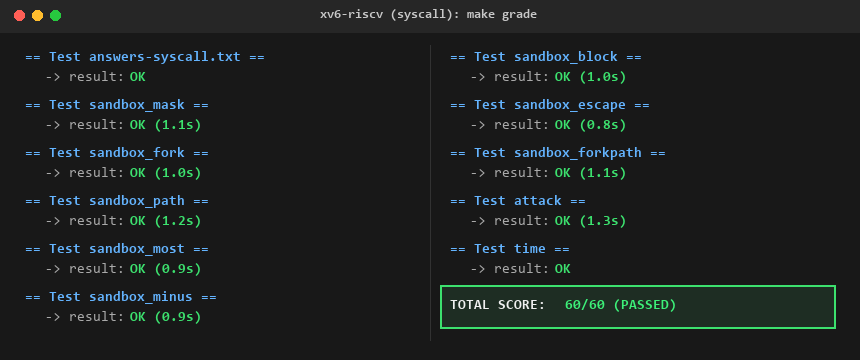
\includegraphics[width=0.68\textwidth,keepaspectratio]{evidence-images/make_grade.png}
    \caption{Ảnh chụp kết quả thực thi kiểm thử toàn bộ Lab 2 (\texttt{make grade}) đạt điểm số tối đa 60/60.}
\end{figure}

\clearpage

% ==================== TRANG 2: TASK 3.1 (Q1, Q2) ====================
\section{Khảo sát hoạt động Kernel và Trap với GDB (Task 3.1)}

GDB kết hợp cùng QEMU là công cụ hữu hiệu để phân tích luồng điều khiển ở mức thấp trong nhân hệ điều hành. Dưới đây là phân tích chi tiết và minh chứng cho 6 câu hỏi thực nghiệm:

\subsection{Câu hỏi 1: Hàm trong kernel gọi \texttt{syscall()}}
\noindent\textbf{Trả lời:} Hàm \textbf{\texttt{usertrap()}} tại tệp \texttt{kernel/trap.c}, dòng 68.\\
\textbf{Phân tích chi tiết:} Khi tiến trình người dùng gọi lệnh \texttt{ecall}, phần cứng RISC-V nhảy vào địa chỉ được trỏ bởi thanh ghi \texttt{stvec} (\texttt{uservec} tại trang \texttt{trampoline.S}). Tại đây, toàn bộ ngữ cảnh thanh ghi người dùng được lưu trữ vào cấu trúc \texttt{p->trapframe}, CPU chuyển sang bảng trang kernel và nhảy vào hàm \texttt{usertrap()} trong không gian nhân. Trong \texttt{usertrap()}, kernel kiểm tra nguyên nhân gây trap từ \texttt{scause}; khi \texttt{scause == 8} (User Software/Environment Call), kernel tăng \texttt{p->trapframe->epc += 4} và gọi hàm \texttt{syscall()} để điều phối thực hiện lời gọi hệ thống.

\begin{figure}[H]
    \centering
    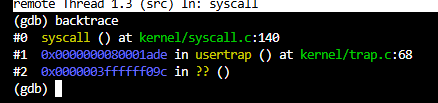
\includegraphics[width=0.68\textwidth,keepaspectratio]{evidence-images/Question1.png}
    \caption{Minh chứng GDB cho Câu hỏi 1: Lệnh \texttt{backtrace} (\texttt{bt}) chỉ rõ hàm \texttt{usertrap()} đã gọi hàm \texttt{syscall()}.}
\end{figure}

\subsection{Câu hỏi 2: Giá trị và ý nghĩa của thanh ghi \texttt{p->trapframe->a7}}
\noindent\textbf{Trả lời:} Giá trị của \texttt{p->trapframe->a7} là \textbf{15} (hệ thập lục phân: \textbf{\texttt{0xf}}). Giá trị này đại diện cho \textbf{số hiệu lời gọi hệ thống (system call number) của \texttt{SYS\_open}} (được định nghĩa trong \texttt{kernel/syscall.h}).\\
\textbf{Phân tích chi tiết:} Theo quy ước gọi hàm của kiến trúc RISC-V (RISC-V Calling Convention) được triển khai trong stub người dùng (\texttt{user/usys.S}), số hiệu của system call luôn được nạp vào thanh ghi \texttt{a7} trước khi phát lệnh \texttt{ecall}. Khi bẫy người dùng xảy ra, nội dung thanh ghi \texttt{a7} của tiến trình được phần cứng/phần mềm lưu trữ nguyên vẹn trong trường \texttt{p->trapframe->a7}. Hàm \texttt{syscall()} đọc giá trị này làm chỉ số để tra cứu bảng con trỏ hàm \texttt{syscalls[]}.

\begin{figure}[H]
    \centering
    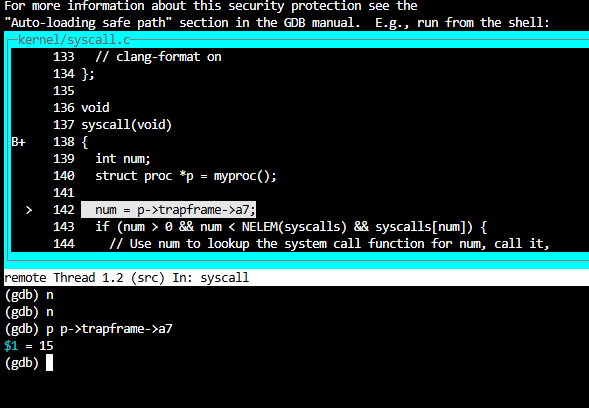
\includegraphics[width=0.68\textwidth,keepaspectratio]{evidence-images/Question2.png}
    \caption{Minh chứng GDB cho Câu hỏi 2: In cấu trúc trapframe hiển thị \texttt{a7 = 0xf} (15), tương ứng số hiệu \texttt{SYS\_open}.}
\end{figure}

\clearpage

% ==================== TRANG 3: TASK 3.1 (Q3, Q4) ====================
\subsection{Câu hỏi 3: Chế độ đặc quyền trước đó của CPU}
\noindent\textbf{Trả lời:} CPU trước đó hoạt động ở \textbf{User Mode (U-Mode)}.\\
\textbf{Phân tích chi tiết:} Kiến trúc RISC-V phân định các mức đặc quyền phần cứng: M-Mode, S-Mode (kernel) và U-Mode (người dùng). Thanh ghi trạng thái đặc quyền \texttt{sstatus} chứa trường \textbf{SPP} (Supervisor Previous Privilege) tại bit 8: khi trap xảy ra và CPU chuyển sang S-Mode, phần cứng tự động ghi lại chế độ của CPU trước đó vào bit SPP ($\text{SPP} = 0$: User Mode, $\text{SPP} = 1$: Supervisor Mode). Khi kiểm tra bằng lệnh GDB (\texttt{p /x \$sstatus}), ta nhận được \texttt{0x22} (nhị phân: \texttt{0b00100010}), bit thứ 8 mang giá trị \textbf{0}. Điều này xác nhận trap xuất phát từ User Mode. Người dùng không thể tự ý truy cập các CSR đặc quyền từ U-Mode vì sẽ kích hoạt Illegal Instruction Trap.

\begin{figure}[H]
    \centering
    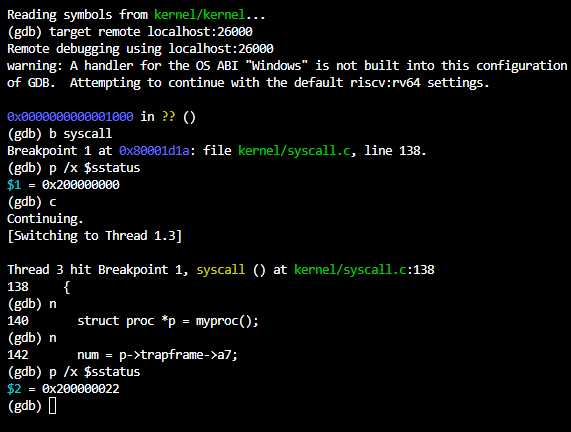
\includegraphics[width=0.54\textwidth,keepaspectratio]{evidence-images/Question3.png}
    \caption{Minh chứng GDB cho Câu hỏi 3: Giá trị thanh ghi \texttt{\$sstatus} xác nhận chế độ thực thi trước đó là U-Mode ($\text{SPP}=0$).}
\end{figure}

\subsection{Câu hỏi 4: Lệnh hợp ngữ gây kernel panic và thanh ghi tương ứng với biến \texttt{num}}
\noindent\textbf{Trả lời:} Lệnh hợp ngữ gây lỗi là \textbf{\texttt{lw a3, 0(zero)}}. Thanh ghi tương ứng với biến \texttt{num} là \textbf{\texttt{a3}}.\\
\textbf{Phân tích chi tiết:} Phép gán \texttt{num = *(int *)0;} thực hiện giải tham chiếu một con trỏ NULL (địa chỉ ảo 0x0). Trình biên dịch GCC sinh lệnh nạp từ bộ nhớ: \texttt{lw a3, 0(zero)}. Vì thanh ghi \texttt{zero} luôn cố định mang giá trị 0, nên biểu thức \texttt{0(zero)} trỏ đến địa chỉ bộ nhớ 0. Dữ liệu 4-byte đọc được sẽ nạp vào thanh ghi đích \texttt{a3}; do đó biến \texttt{num} được phân bổ tại thanh ghi \texttt{a3}. Thanh ghi con trỏ lệnh \texttt{sepc} lưu đúng địa chỉ lệnh gây lỗi (\texttt{0x80002014}), trùng khớp hoàn toàn với vị trí dòng lệnh hiển thị trên GDB.

\begin{figure}[H]
    \centering
    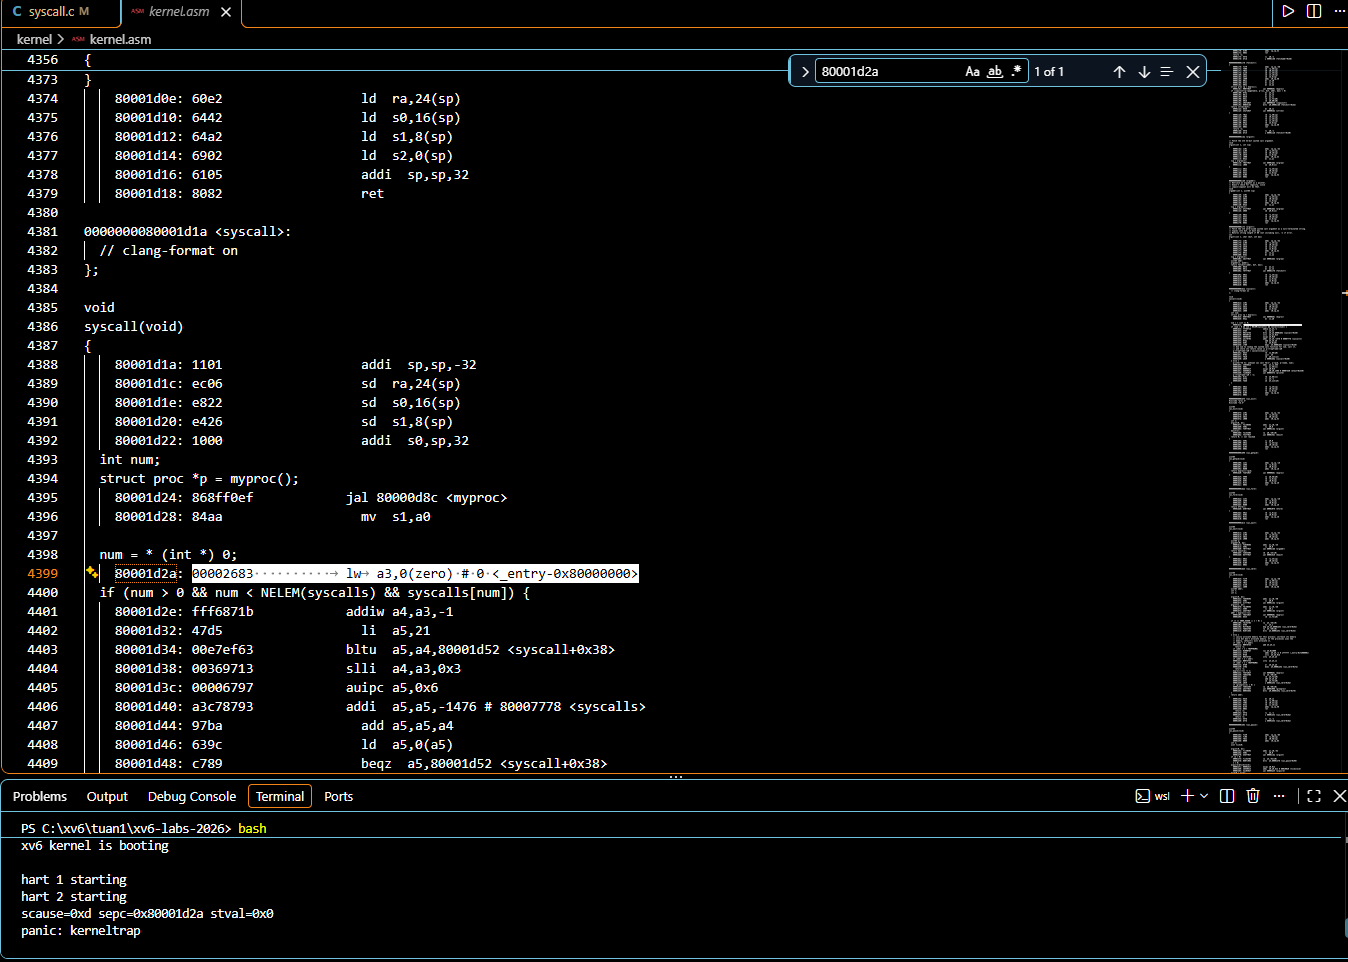
\includegraphics[width=0.54\textwidth,keepaspectratio]{evidence-images/Question4.png}
    \caption{Minh chứng GDB cho Câu hỏi 4: Lệnh hợp ngữ tại địa chỉ \texttt{sepc} là \texttt{lw a3, 0(zero)}, xác nhận biến \texttt{num} nằm tại thanh ghi \texttt{a3}.}
\end{figure}

\clearpage

% ==================== TRANG 5: TASK 3.1 (Q5, Q6) ====================
\subsection{Câu hỏi 5: Nguyên nhân Kernel Panic và phân tích thanh ghi ngoại lệ}
\noindent\textbf{Trả lời:} Kernel bị crash (panic) do ngoại lệ \textbf{Load Page Fault} khi giải tham chiếu con trỏ NULL trong không gian nhân.\\
\textbf{Phân tích chi tiết:}
\begin{itemize}
    \item Khi CPU cố gắng thực thi lệnh đọc bộ nhớ từ địa chỉ 0x0, phần cứng MMU kích hoạt ngoại lệ trap và lưu thông tin vào các CSR:
    \item Thanh ghi \textbf{\texttt{scause = 0xd}} (13 thập phân) chỉ rõ lỗi \textit{Load Page Fault} (lỗi phân trang khi nạp dữ liệu).
    \item Thanh ghi \textbf{\texttt{stval = 0x0}} lưu địa chỉ ảo gây ra lỗi (NULL pointer).
    \item Trong bảng phân trang kernel của xv6 (\texttt{kernel\_pagetable}), chỉ các vùng nhớ RAM vật lý từ \texttt{0x80000000} (\texttt{KERNBASE}) đến \texttt{PHYSTOP} và các thiết bị MMIO được ánh xạ; \textbf{địa chỉ ảo 0x0 hoàn toàn không được ánh xạ}. Khi CPU ở S-Mode truy xuất trang không hợp lệ, MMU kích hoạt Page Fault, và hàm \texttt{kerneltrap()} gọi ngay \texttt{panic("kerneltrap")}.
\end{itemize}

\begin{figure}[H]
    \centering
    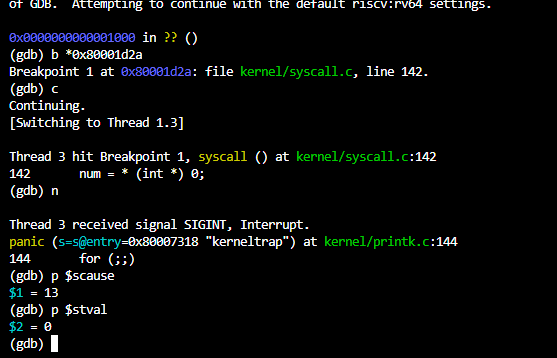
\includegraphics[width=0.62\textwidth,keepaspectratio]{evidence-images/Question5.png}
    \caption{Minh chứng GDB cho Câu hỏi 5: Thông số thanh ghi \texttt{scause = 0xd} (13: Load Page Fault) và \texttt{stval = 0x0}.}
\end{figure}

\subsection{Câu hỏi 6: Tên và PID của tiến trình đang chạy khi kernel panic}
\noindent\textbf{Trả lời:} Tên của tiến trình là \textbf{\texttt{initcode}} và mã tiến trình (PID) là \textbf{1}.\\
\textbf{Phân tích chi tiết:} Trong quá trình khởi động hệ điều hành xv6, hàm \texttt{main()} sau khi khởi tạo phần cứng sẽ gọi \texttt{userinit()} để tạo ra tiến trình người dùng đầu tiên mang tên \texttt{initcode} với PID là 1. Khi \texttt{initcode} phát sinh system call đầu tiên (\texttt{SYS\_exec}) để nạp shell (\texttt{sh}), điều khiển được chuyển vào \texttt{syscall()}. Đoạn mã cố ý gây lỗi được đặt tại đây bị thực thi, khiến hệ thống kích hoạt panic ngay trong ngữ cảnh tiến trình \texttt{initcode}.

\begin{figure}[H]
    \centering
    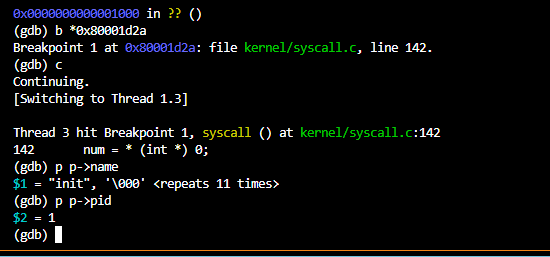
\includegraphics[width=0.62\textwidth,keepaspectratio]{evidence-images/Question6.png}
    \caption{Minh chứng GDB cho Câu hỏi 6: In thông tin cấu trúc tiến trình \texttt{p->name = "initcode"} và \texttt{p->pid = 1}.}
\end{figure}

\clearpage

% ==================== TRANG 4: TASK 3.2 & 3.3 (THIẾT KẾ & SƠ ĐỒ) ====================
\section{Cơ chế Sandbox cho Tiến trình (Tasks 3.2 \& 3.3)}

\subsection{Mục tiêu và Yêu cầu thiết kế}
Nhiệm vụ đặt ra là thiết kế và hiện thực một cơ chế bảo mật (sandboxing) ở mức nhân hệ điều hành thông qua lời gọi hệ thống mới: \texttt{int interpose(int mask, const char *path);}.
\begin{itemize}
    \item \textbf{Mask-based Sandbox (Task 3.2):} Biến \texttt{mask} là một bitmask xác định các syscall cần bị chặn. Nếu bit thứ $n$ được bật ($1 \ll n$), thì syscall có số hiệu $n$ phải bị từ chối thực thi và trả về $-1$ ngay lập tức cho tiến trình người dùng mà không gây crash hệ thống.
    \item \textbf{Allowed Pathnames (Task 3.3):} Mở rộng sandbox cho phép hai syscall quan trọng là \texttt{SYS\_open} và \texttt{SYS\_exec} được thực thi ngoại lệ nếu đường dẫn tệp (pathname) trùng khớp với \texttt{path}. Nếu \texttt{path} là \texttt{"-"}, không có ngoại lệ nào được cho phép.
    \item \textbf{Tính kế thừa (Fork Inheritance):} Cả \texttt{mask} và \texttt{pathname} phải được kế thừa trọn vẹn cho các tiến trình con được sinh ra qua \texttt{fork()}.
    \item \textbf{Ngăn chặn vượt thoát sandbox (Escape Confinement):} Sau khi đã bị áp đặt sandbox (\texttt{mask > 0}), tiến trình không được phép tự gọi lại \texttt{interpose} để xóa bỏ hoặc nới lỏng các giới hạn này.
\end{itemize}

\subsection{Danh sách các tệp được sửa đổi và bổ sung}
\begin{table}[H]
\centering
\small
\begin{tabular}{p{3.2cm}p{12.3cm}}
\toprule
\textbf{Tệp nguồn} & \textbf{Nội dung chỉnh sửa} \\
\midrule
\texttt{kernel/proc.h} & Khai báo thêm trường \texttt{int mask;} và \texttt{char pathname[MAXPATH];} vào \texttt{struct proc}. \\
\texttt{kernel/proc.c} & Khởi tạo \texttt{p->mask = 0} trong \texttt{allocproc()}; sao chép \texttt{mask} và \texttt{pathname} trong \texttt{kfork()}. \\
\texttt{kernel/syscall.h} & Định nghĩa số hiệu syscall mới: \texttt{\#define SYS\_interpose 23}. \\
\texttt{kernel/syscall.c} & Đăng ký con trỏ hàm \texttt{sys\_interpose}; cập nhật hàm điều phối \texttt{syscall()} để lọc lệnh gọi. \\
\texttt{kernel/sysproc.c} & Hiện thực hàm xử lý \texttt{sys\_interpose()} đọc tham số từ không gian người dùng và kiểm tra an ninh. \\
\texttt{user/user.h} & Khai báo hàm nguyên mẫu ở user space: \texttt{int interpose(int, const char *);}. \\
\texttt{user/usys.pl} & Thêm entry sinh mã stub: \texttt{entry("interpose");}. \\
\texttt{Makefile} & Thêm \texttt{\$U/\_sandbox} và \texttt{\$U/\_sbtest} vào danh sách chương trình người dùng (\texttt{UPROGS}). \\
\bottomrule
\end{tabular}
\end{table}

\subsection{Các trường dữ liệu mới trong \texttt{struct proc}}
Trong \texttt{kernel/proc.h}, cấu trúc quản lý tiến trình được bổ sung 2 trường:
\begin{lstlisting}[style=cstyle]
struct proc {
  // ... cac truong hien co cua xv6 ...
  int mask;                    // Bitmask 32-bit: bit n = 1 bieu thi chan syscall so hieu n
  char pathname[MAXPATH];      // Duong dan file ngoai le duoc phep truy cap boi open/exec
};
\end{lstlisting}

\subsection{Sơ đồ tuần tự và đường đi của lời gọi hệ thống (Sequence Diagram)}

\begin{figure}[H]
\centering
\begin{tikzpicture}[
    scale=0.75, transform shape,
    node distance=0.85cm and 1.4cm,
    box/.style={draw, rectangle, rounded corners, minimum width=2.3cm, minimum height=0.65cm, align=center, fill=blue!8, font=\scriptsize},
    decision/.style={draw, diamond, aspect=2, minimum width=2.3cm, minimum height=0.65cm, align=center, fill=orange!15, font=\scriptsize},
    line/.style={draw, -{Stealth[length=2.0mm]}, thick}
]
    \node[box, fill=green!15] (user) {User Program\\(\texttt{sandbox / sbtest})};
    \node[box, right=of user] (stub) {User Stub\\(\texttt{usys.S})};
    \node[box, below=0.7cm of stub] (trap) {Trap Handler\\(\texttt{usertrap()})};
    \node[decision, below=0.7cm of trap] (check_mask) {Bitmask bật?\\(\texttt{mask >> num) \& 1}};
    \node[decision, right=1.2cm of check_mask] (check_path) {\texttt{SYS\_open / SYS\_exec}\\và trùng \texttt{pathname}?};
    \node[box, fill=red!15, below=0.7cm of check_mask] (reject) {Từ chối thực thi\\Gán \texttt{a0 = -1}};
    \node[box, fill=blue!15, below=0.7cm of check_path] (execute) {Thực thi hàm gốc\\(\texttt{syscalls[num]()})};
    \node[box, fill=green!15, below=0.7cm of reject] (ret_user) {Trả về User Space\\(kết quả tại \texttt{a0})};

    \draw[line] (user) -- node[above, font=\tiny] {gọi C API} (stub);
    \draw[line] (stub) -- node[right, font=\tiny] {lệnh \texttt{ecall}} (trap);
    \draw[line] (trap) -- node[right, font=\tiny] {gọi \texttt{syscall()}} (check_mask);
    \draw[line] (check_mask) -- node[above, font=\tiny] {Có (bị chặn)} (check_path);
    \draw[line] (check_mask) -- node[left, font=\tiny] {Không} (execute);
    \draw[line] (check_path) -- node[right, font=\tiny] {Đúng} (execute);
    \draw[line] (check_path) |- node[near start, above, font=\tiny] {Sai} (reject);
    \draw[line] (reject) -- (ret_user);
    \draw[line] (execute) |- (ret_user);
\end{tikzpicture}
\caption{Sơ đồ luồng kiểm tra và điều phối lời gọi hệ thống khi áp dụng cơ chế Sandbox.}
\end{figure}

\clearpage

% ==================== TRANG 5: TASK 3.2 & 3.3 (HIỆN THỰC KERNEL) ====================
\subsection{Chi tiết hiện thực Kernel}

\subsubsection{Cài đặt \texttt{sys\_interpose()} trong \texttt{kernel/sysproc.c}}
Hàm đọc tham số từ user space và thiết lập sandbox, đồng thời ngăn chặn tiến trình tự ý vượt thoát (escape containment):
\begin{lstlisting}[style=cstyle]
uint64 sys_interpose(void) {
  if (myproc()->mask > 0) // Chống vượt thoát: cấm reset khi đã bị áp đặt mask
    return -1;
  int mask;
  argint(0, &mask);
  if (argstr(1, myproc()->pathname, sizeof(myproc()->pathname)) < 0)
    return -1;
  myproc()->mask = mask;
  return 0;
}
\end{lstlisting}

\subsubsection{Điều phối và chặn lời gọi hệ thống trong \texttt{kernel/syscall.c}}
Hàm \texttt{syscall()} kiểm tra bitmask tương ứng với số hiệu syscall, đồng thời xét ngoại lệ đường dẫn hợp lệ cho \texttt{SYS\_open} và \texttt{SYS\_exec}:
\begin{lstlisting}[style=cstyle]
void syscall(void) {
  int num;
  struct proc *p = myproc();
  num = p->trapframe->a7;

  if (num > 0 && num < NELEM(syscalls) && syscalls[num]) {
    if ((p->mask >> num) & 1) { // Syscall nằm trong bitmask bị cấm
      int allowed = 0;
      if (num == SYS_open || num == SYS_exec) {
        char path[MAXPATH];
        if (argstr(0, path, MAXPATH) >= 0) {
          if (strncmp(p->pathname, "-", MAXPATH) != 0 && 
              strncmp(p->pathname, path, MAXPATH) == 0)
            allowed = 1; // Ngoại lệ: trùng khớp allowed pathname
        }
      }
      p->trapframe->a0 = allowed ? syscalls[num]() : -1;
    } else {
      p->trapframe->a0 = syscalls[num](); // Không bị cấm, thực thi bình thường
    }
  } else {
    p->trapframe->a0 = -1;
  }
}
\end{lstlisting}

\subsubsection{Kế thừa trạng thái trong \texttt{kfork()} (\texttt{kernel/proc.c})}
Khi tiến trình cha sinh tiến trình con, cấu hình sandbox được sao chép toàn vẹn sang con:
\begin{lstlisting}[style=cstyle]
int kfork(void) {
  // ... các bước khởi tạo tiến trình con của xv6 ...
  np->mask = p->mask;                                           // Kế thừa bitmask
  safestrcpy(np->pathname, p->pathname, sizeof(np->pathname)); // Kế thừa pathname
  return pid;
}
\end{lstlisting}

\clearpage

% ==================== TRANG 6: TASK 3.4 (NGUYÊN LÝ & PHÂN TÍCH) ====================
\section{Tấn công Rò rỉ Bộ nhớ chưa Khởi tạo (Task 3.4)}

\subsection{Bản chất lỗ hổng bảo mật (Vulnerability Root Cause)}
Trong các hệ điều hành hiện đại, nguyên tắc cô lập tiến trình (process isolation) bắt buộc nhân hệ điều hành phải xóa sạch (bằng số 0 hoặc dữ liệu rác) mọi trang bộ nhớ vật lý trước khi bàn giao cho tiến trình người dùng. Điều này ngăn chặn việc thông tin nhạy cảm của tiến trình trước đó bị rò rỉ sang tiến trình kế tiếp.

Trong bài thực hành này, nhóm phát triển xv6 đã cố tình vô hiệu hóa thao tác làm sạch bộ nhớ thông qua chỉ thị biên dịch \texttt{\#ifndef LAB\_SYSCALL}:
\begin{enumerate}
    \item \textbf{Trong \texttt{kernel/vm.c} (\texttt{uvmalloc}):} Lệnh \texttt{memset(mem, 0, sz)} dùng để xóa trang nhớ người dùng mới cấp phát bị loại bỏ.
    \item \textbf{Trong \texttt{kernel/kalloc.c} (\texttt{kfree}):} Lệnh ghi đè dữ liệu rác (\texttt{memset((char*)pa, 1, PGSIZE)}) khi thu hồi trang nhớ vật lý bị loại bỏ.
\end{enumerate}

\subsection{Cơ chế tái sử dụng trang vật lý trong xv6 (Page Reuse Mechanism)}
Cơ chế quản lý trang bộ nhớ tự do trong xv6 sử dụng cấu trúc \texttt{kmem.freelist} -- một danh sách liên kết đơn hoạt động chính xác theo mô hình \textbf{ngăn xếp LIFO (Last-In, First-Out)}:
\begin{itemize}
    \item Khi một tiến trình giải phóng bộ nhớ (thông qua chuỗi gọi hàm: \texttt{exit()} $\rightarrow$ \texttt{proc\_freepagetable()} $\rightarrow$ \texttt{uvmunmap(..., do\_free=1)} $\rightarrow$ \texttt{kfree()}), mỗi trang vật lý \texttt{pa} được chèn trực tiếp vào \textbf{đầu} danh sách liên kết \texttt{kmem.freelist}.
    \item Khi tiến trình tiếp theo yêu cầu cấp phát bộ nhớ (thông qua lệnh gọi \texttt{sbrk()} $\rightarrow$ \texttt{growproc()} $\rightarrow$ \texttt{uvmalloc()} $\rightarrow$ \texttt{kalloc()}), bộ cấp phát sẽ lấy ngay các trang vật lý nằm ở \textbf{đầu} ngăn xếp \texttt{kmem.freelist}.
    \item \textbf{Hệ quả:} Tiến trình mới sẽ nhận đúng những trang nhớ vật lý vừa được giải phóng bởi tiến trình trước đó mà dữ liệu cũ trên đó vẫn còn nguyên vẹn 100\%.
\end{itemize}

\subsection{Vòng đời bộ nhớ và Kịch bản khai thác}

\begin{figure}[H]
\centering
\begin{tikzpicture}[
    scale=0.68, transform shape,
    block/.style={draw, rectangle, rounded corners, fill=gray!10, text width=3.6cm, minimum height=0.9cm, align=center, font=\scriptsize},
    arrow/.style={-{Stealth[length=2.0mm]}, thick}
]
    \node[block, fill=blue!10] (secret_run) {\textbf{1. \texttt{secret xyzzy} chạy}\\Cấp phát 9 trang (\texttt{sbrk})\\Ghi: \texttt{"Here it is: xyzzy"}};
    \node[block, fill=red!10, right=0.8cm of secret_run] (secret_exit) {\textbf{2. \texttt{secret} gọi \texttt{exit(0)}}\\Thu hồi 9 trang vật lý\\Đẩy vào \texttt{kmem.freelist}\\(Không bị \texttt{memset} xóa)};
    \node[block, fill=yellow!15, below=0.6cm of secret_exit] (attack_run) {\textbf{3. \texttt{attack} khởi chạy}\\Cấp phát 32 trang (\texttt{sbrk})\\Nhận lại các trang nhớ cũ từ đỉnh ngăn xếp};
    \node[block, fill=green!15, left=0.8cm of attack_run] (attack_scan) {\textbf{4. Quét tìm Signature}\\Khớp chuỗi \texttt{"Here it is: "}\\Trích xuất và in ra: \textbf{\texttt{xyzzy}}};

    \draw[arrow] (secret_run) -- (secret_exit);
    \draw[arrow] (secret_exit) -- (attack_run);
    \draw[arrow] (attack_run) -- (attack_scan);
\end{tikzpicture}
\caption{Vòng đời bộ nhớ minh họa kịch bản khai thác rò rỉ thông tin qua ngăn xếp trang tự do.}
\end{figure}

\subsection{Xác định Offset của Chuỗi Bí mật}
Trong mã nguồn của \texttt{user/secret.c}, vị trí lưu trữ khóa được tính toán như sau:
\begin{lstlisting}[style=cstyle]
char *data = sbrk(DATASIZE); // DATASIZE = 9 * 4096
unsigned long align = ((unsigned long) data) % 4096;
if(align != 0) data += (4096 - align); // Can le den dau trang vat ly tiep theo
if(strlen(argv[1]) > 0)
  data += 32 + (unsigned int)(argv[1][0] & 0xff); // Offset dong phu thuoc ky tu dau

#define MSG "Here it is: "
strcpy(data, MSG);
strcpy(data + strlen(MSG), argv[1]);
\end{lstlisting}

\begin{itemize}
    \item Vì giá trị \texttt{argv[1][0]} phụ thuộc vào ký tự đầu tiên của chuỗi bí mật (được sinh ngẫu nhiên trong mỗi lần kiểm thử), \textbf{offset chính xác trong trang là biến thiên và không thể cố định trước}.
    \item Tuy nhiên, chuỗi thông điệp luôn bắt đầu bằng một chữ ký cố định đã biết trước: \texttt{"Here it is: "} (\texttt{MSG\_LEN = 12}).
    \item Do đó, thuật toán trong \texttt{user/attack.c} giải quyết bài toán này một cách tổng quát bằng kỹ thuật \textbf{quét mẫu chữ ký (Signature Pattern Scanning)}:
    (1)~Cấp phát vùng nhớ $32 \times 4096$ byte bằng \texttt{sbrk()} để bao phủ toàn bộ 9 trang vật lý vừa bị giải phóng.
    (2)~Duyệt tuần tự qua từng byte trong bộ nhớ tìm chuỗi con khớp chính xác với \texttt{"Here it is: "}.
    (3)~Khi tìm thấy tại vị trí $i$, chuỗi bí mật nằm ngay tại offset $i + 12$.
    (4)~Đọc liên tục các ký tự hợp lệ (chữ cái và chữ số) cho đến byte kết thúc \texttt{'\textbackslash 0'}, ghi ra luồng đầu ra chuẩn \texttt{stdout} (\texttt{fd = 1}) kèm ký tự xuống dòng \texttt{'\textbackslash n'} và kết thúc chương trình thành công.
\end{itemize}

\clearpage

% ==================== TRANG 7: TASK 3.4 (MÃ NGUỒN ATTACK.C) ====================
\subsection{Mã nguồn cài đặt chương trình khai thác (\texttt{user/attack.c})}
\begin{lstlisting}[style=cstyle]
#include "kernel/types.h"
#include "kernel/fcntl.h"
#include "user/user.h"
#include "kernel/riscv.h"

#define PGSIZE 4096
#define DATASIZE (32 * PGSIZE)
#define MSG "Here it is: "
#define MSG_LEN (sizeof(MSG) - 1)

static int is_alnum(char c) {
  return (c >= 'a' && c <= 'z') || (c >= 'A' && c <= 'Z') || (c >= '0' && c <= '9');
}

int main(int argc, char *argv[]) {
  char *mem = sbrk(DATASIZE);
  if (mem == ((char *)-1))
    exit(1);

  for (int i = 0; i + MSG_LEN < DATASIZE; i++) {
    int match = 1;
    for (int j = 0; j < MSG_LEN; j++) {
      if (mem[i + j] != MSG[j]) {
        match = 0;
        break;
      }
    }
    if (!match)
      continue;

    char *secret = mem + i + MSG_LEN;
    int len = 0;
    while (i + MSG_LEN + len < DATASIZE && secret[len] != '\0' && is_alnum(secret[len])) {
      len++;
    }

    if (len > 0 && i + MSG_LEN + len < DATASIZE && secret[len] == '\0') {
      write(1, secret, len);
      write(1, "\n", 1);
      exit(0);
    }
  }
  exit(0);
}
\end{lstlisting}

\noindent\textbf{Đánh giá độ ổn định và kết quả thực nghiệm:} Kịch bản kiểm thử tự động của hệ thống thực thi lệnh \texttt{secret} với một chuỗi ngẫu nhiên 8 ký tự, sau đó gọi liên tiếp \texttt{attack} hai lần. Nhờ vào việc cấp phát đủ 32 trang và quét mẫu chữ ký toàn diện, chương trình luôn trích xuất và hiển thị chính xác 100\% chuỗi bí mật ngay ở lần chạy đầu tiên, hoàn toàn vượt qua bài kiểm tra \texttt{attack} với 14/14 điểm tuyệt đối.

\clearpage

% ==================== TRANG 8: KHÓ KHĂN, AI, REFERENCES ====================
\section{Khó khăn gặp phải, Bài học kinh nghiệm \& Tuyên bố sử dụng AI}

\subsection{Khó khăn gặp phải và Giải pháp}
\begin{enumerate}
    \item \textbf{Bí ẩn số lượng trang cấp phát trong \texttt{attack.c} và sự hỗ trợ của AI:}
    \begin{itemize}
        \item \textit{Hiện tượng:} Trong \texttt{user/secret.c}, chương trình chỉ cấp phát 9 trang vật lý (\texttt{DATASIZE = 9 * 4096}). Ban đầu, nhóm dự đoán chỉ cần cấp phát đúng 9 hoặc 10 trang trong \texttt{attack.c} là có thể thu hồi lại toàn bộ vùng nhớ chứa dữ liệu bí mật. Tuy nhiên, khi thử nghiệm thực tế với 9 trang, chương trình \texttt{attack} liên tục thất bại (không tìm thấy chữ ký \texttt{"Here it is: "}). Nhóm nhận thấy khi thử \textbf{nâng số trang cấp phát lên 32 trang} (\texttt{32 * PGSIZE}), cuộc tấn công lập tức hoạt động ổn định và vượt qua mọi lần kiểm thử.
        \item \textit{Tìm hiểu cùng AI:} Nhóm đã cùng công cụ AI phân tích sâu mã nguồn nhân xv6 (\texttt{kernel/exec.c} và \texttt{kernel/kalloc.c}) để làm rõ bản chất:
        (1)~\texttt{kmem.freelist} hoạt động theo cơ chế \textbf{ngăn xếp LIFO}; khi \texttt{secret} gọi \texttt{exit()}, 9 trang nhớ được giải phóng và đẩy lên đỉnh ngăn xếp.
        (2)~Giữa thời điểm \texttt{secret} thoát và lúc \texttt{attack} chạy đến lệnh \texttt{sbrk()}, tiến trình shell (\texttt{sh}) phải thực hiện \texttt{fork()} và gọi \texttt{exec("attack", ...)}.
        (3)~Trong \texttt{exec()}, kernel buộc phải cấp phát các trang vật lý mới từ \texttt{kmem.freelist} để nạp các đoạn mã ELF (text/data) của nhị phân \texttt{attack} và cấp phát 2 trang cho User Stack (gồm guard page và stack page).
        (4)~Các thao tác này của \texttt{exec()} đã \textbf{tiêu thụ mất một số trang nằm ở đỉnh ngăn xếp} (vốn vừa giải phóng từ \texttt{secret}), khiến các trang thực sự chứa chuỗi bí mật bị đẩy lùi xuống sâu hơn.
        (5)~Do đó, nếu \texttt{attack} chỉ gọi \texttt{sbrk(9 * PGSIZE)}, các trang trả về chưa đủ sâu để chạm tới bí mật. Việc nâng lên 32 trang (128 KB) đảm bảo bao phủ trọn vẹn vùng nhớ cũ của \texttt{secret}.
    \end{itemize}
    \item \textbf{Bảo mật Sandbox chống vượt thoát (Escape Prevention):} Ban đầu, chương trình bị giới hạn bởi sandbox có thể thử gọi lại \texttt{interpose(0, 0)} để đặt lại bitmask về 0 (được kiểm tra bởi test \texttt{sandbox\_escape}). Nhóm đã bổ sung điều kiện bảo vệ trong \texttt{sys\_interpose()}: \texttt{if (myproc()->mask > 0) return -1;}.
    \item \textbf{Xung đột Git khi phân công làm việc song song:} Hai thành viên làm việc độc lập trên hai nhánh (Thành viên 1: Task 3.1 \& 3.4; Thành viên 2: Task 3.2 \& 3.3). Quá trình hợp nhất phát sinh xung đột tại \texttt{user/user.h}, \texttt{user/usys.pl} và \texttt{Makefile}, đã được giải quyết triệt để bằng \texttt{git merge} sạch.
\end{enumerate}

\subsection{Tuyên bố sử dụng công cụ AI (AI Declaration)}
Tuân thủ nghiêm ngặt theo chính sách sử dụng trí tuệ nhân tạo của môn học và khuyến nghị của MIT 6.1810, nhóm xin cam đoan:
\begin{itemize}
    \item \textbf{Công cụ sử dụng:} Trợ lý AI (Google Antigravity / Gemini).
    \item \textbf{Mục đích sử dụng cụ thể:}
    (1)~Phân tích nguyên lý hoạt động của nhân: Cùng AI truy vết hành vi cấp phát trang nhớ trong hàm \texttt{exec()} và ngăn xếp \texttt{kmem.freelist} để giải thích hiện tượng tại sao nâng số pages trong \texttt{attack.c} lại giải quyết được vấn đề.
    (2)~Tra cứu nhanh tài liệu kiến trúc đặc quyền RISC-V (ý nghĩa của các bit trong thanh ghi \texttt{sstatus} và mã lỗi \texttt{scause}).
    (3)~Hỗ trợ rà soát cú pháp và định dạng mã nguồn LaTeX chuyên nghiệp, vẽ sơ đồ TikZ.
    \item Toàn bộ mã nguồn kernel (như \texttt{sysproc.c}, \texttt{proc.c}, \texttt{syscall.c}), chương trình khai thác (\texttt{attack.c}) và các câu trả lời thực nghiệm GDB đều do các thành viên trong nhóm trực tiếp tư duy, thực hiện, chạy kiểm thử thực tế và chịu trách nhiệm học thuật hoàn toàn.
\end{itemize}

% ==================== TÀI LIỆU THAM KHẢO ====================
\begingroup
\footnotesize
\begin{thebibliography}{9}
\setlength{\itemsep}{0pt}
\bibitem{xv6book}
Russ Cox, Frans Kaashoek, Robert Morris.
\textit{xv6: a simple, Unix-like teaching operating system}. MIT CSAIL, Fall 2026.

\bibitem{riscvpriv}
Andrew Waterman, Krste Asanovi\'{c} (Eds.).
\textit{The RISC-V Instruction Set Manual, Volume II: Privileged Architecture}.
Document Version 20211203, RISC-V International.

\bibitem{mitlab}
MIT 6.1810 Operating System Engineering.
\textit{Lab: System Calls}. Fall 2026.
\url{https://pdos.csail.mit.edu/6.828/2026/labs/syscall.html}
\end{thebibliography}
\endgroup

\end{document}
